\documentclass{article}

\usepackage[portuges]{babel}
%\usepackage{hyperref}
\usepackage{graphicx}
\usepackage{amsmath}
\usepackage[hidelinks]{hyperref}
 \usepackage{url}
 \usepackage{listings}

\graphicspath{ {./images/} }


\begin{document}

\title{Power PCB outline}
\author{Ian Downie}
\date{May 2024}
\maketitle



\newpage
\section{Introduction}

The purpose of this document is to outline the creation of our first prototype for the data buoy's power electronics in order to facilitate its future development.

\section{Summary of functions and schematic}

The essential functions that this prototype is designed to fulfil are pseudo-MPPT for PV panels, battery management and voltage regulation for the MCU, communications, data storage and instrumentation, which are summarised in Figure \ref{fig:mesh1}. This report will describe how these functions have been implemented by starting at the input of energy from the PV panels until the regulated voltage outputs.

\begin{figure}[h]
	\centering
   	 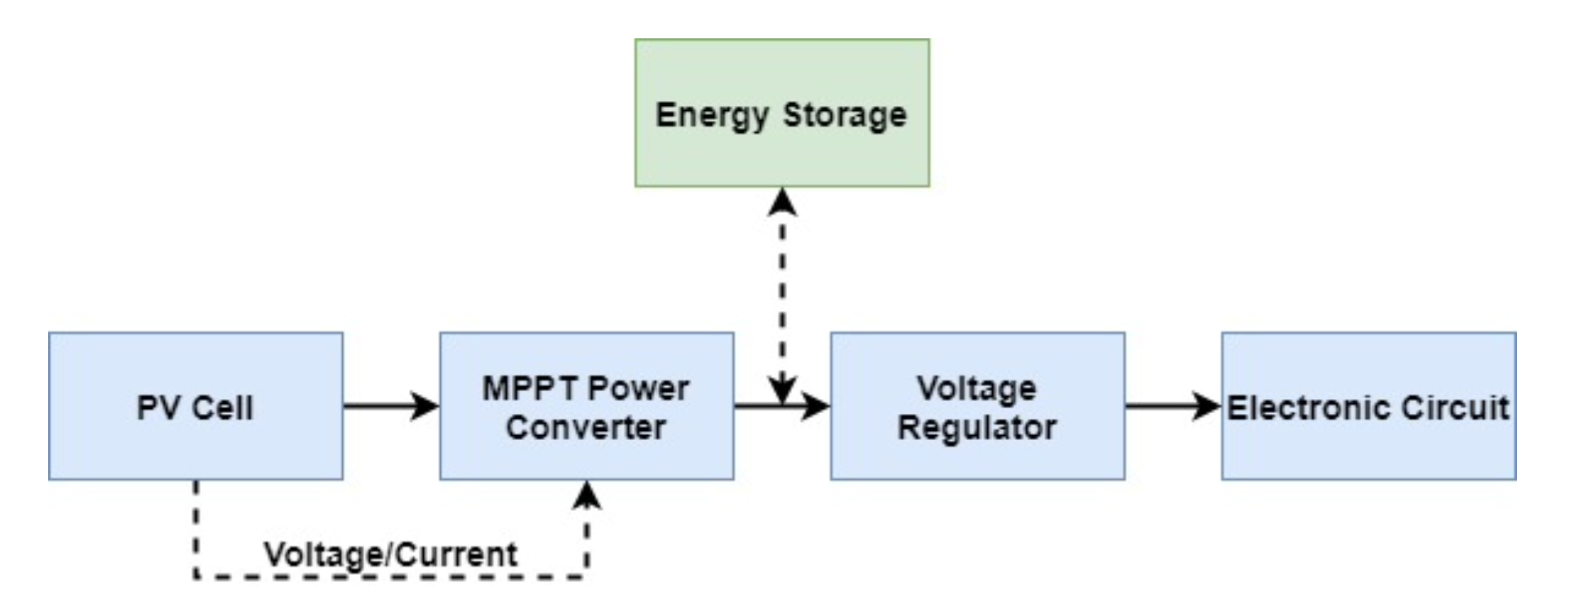
\includegraphics[width=\linewidth]{Energy-Storage}
	\caption{Overview of power architecture}
	\label{fig:mesh1}
\end{figure}



\subsection{Solar panel connection}

The design of the buoy's hull allows for the installation of six custom-built PV panels. Each panel will provide a nominal MPP voltage of approximately 6V and the PCB PV-panel connections are made so that the panels are in parallel and the resultant voltage of each panel is the MPP, described in a later section, while the current provided by the panels is the sum of the currents from the panels. In operation, the six panels will never be fully exposed to the sun. Even with the sun at its zenith, when all six panels will be contributing a reasonable current, they will not be operation at full power output due to the inclination of the panels. 

A barrel jack as been provided for each PV panel to connect to the PCB. In accordance with the recommendation of our MPPT IC, the BQ24650 from Texas Instruments, a damping RC circuit is configured on the positive pin of the barrel jack in order to suppress spikes that may appear from hot plug-in oscillation. A diode is also placed on each PV-panel input to prevent reverse current from both the MPPT IC and the other solar panel inputs that may be operating at a higher voltage level. An additional damping RC circuit is placed near the MPPT IC. Please see Figure \ref{fig:mesh2} for the datasheet schematic as well as its implmentation on our PCB.

\begin{figure}[h]
	\centering
   	 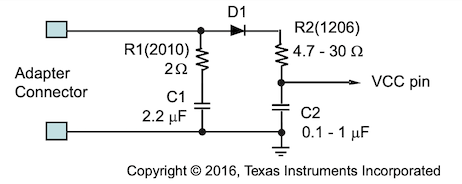
\includegraphics[scale = 1]{TI-filter}
   	 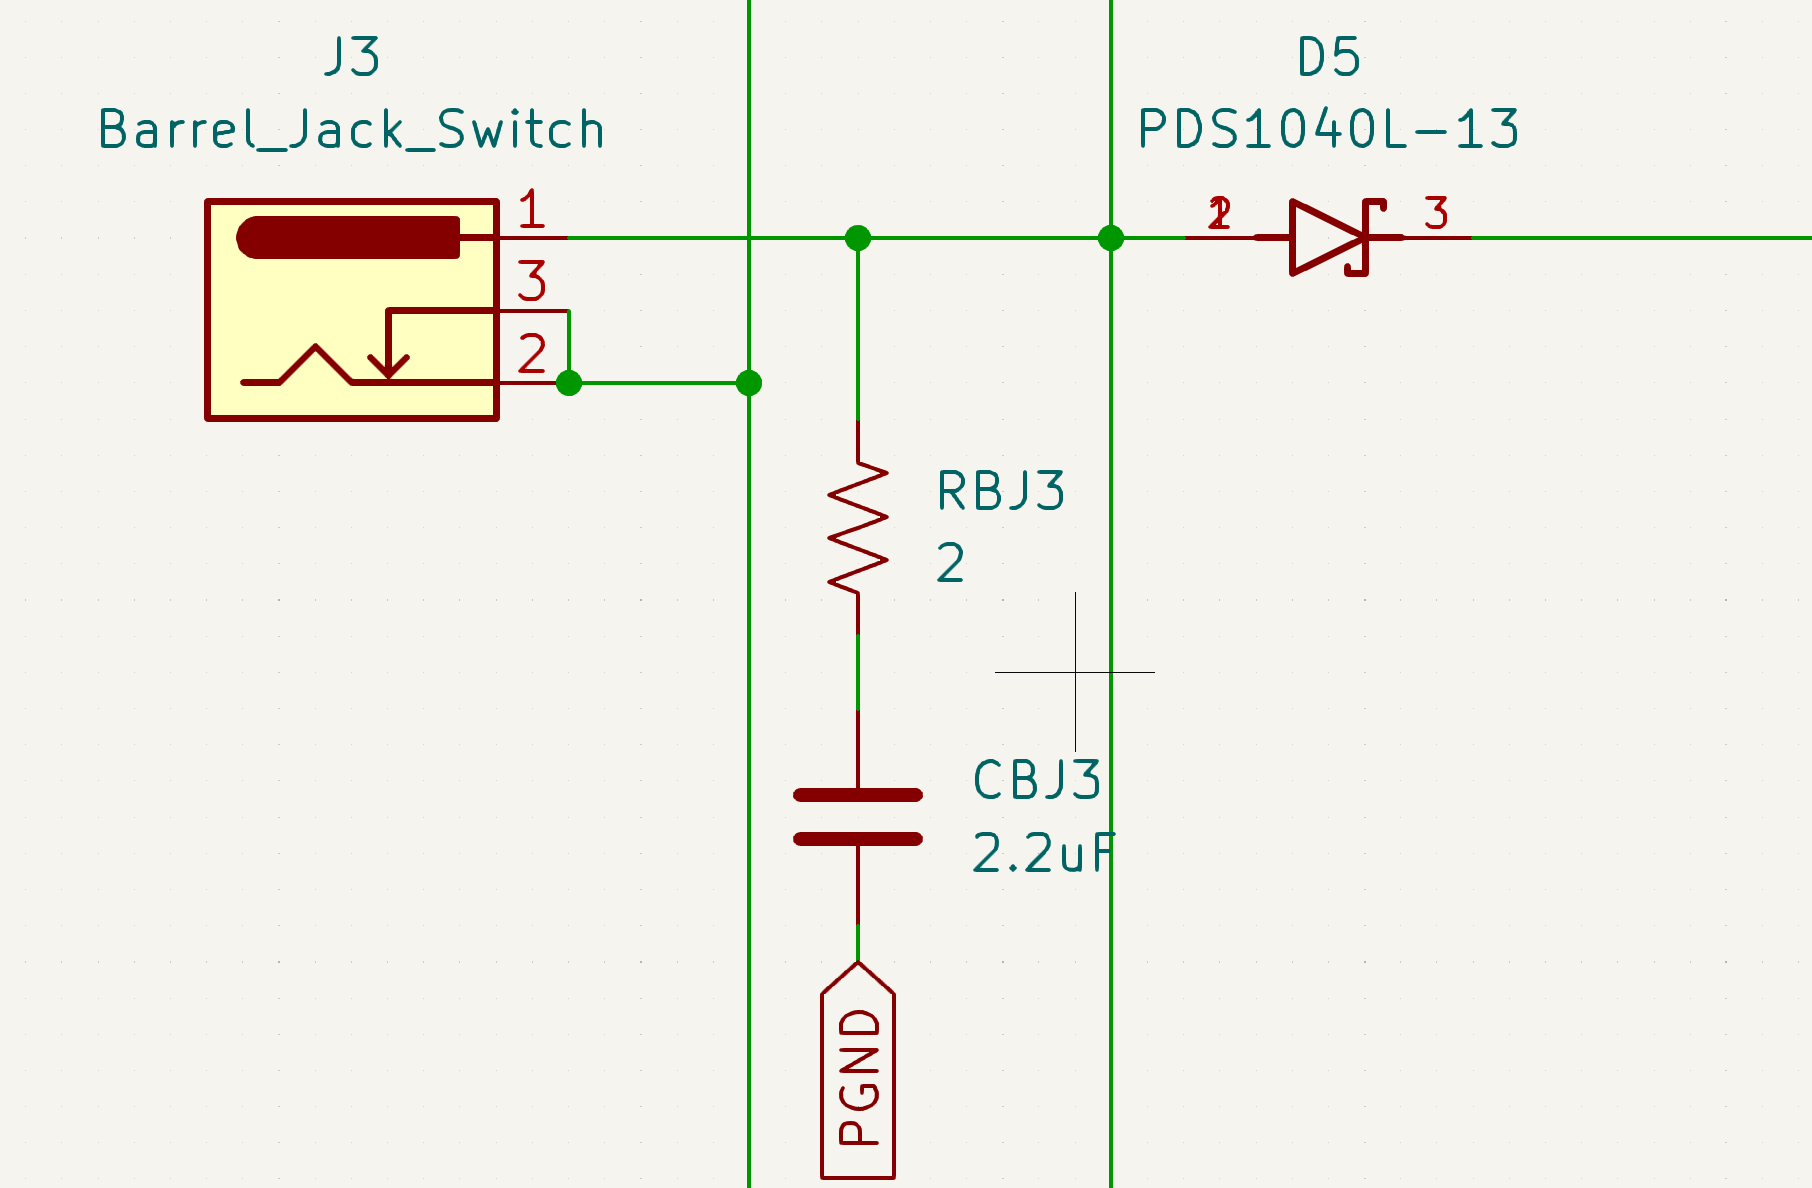
\includegraphics[scale = 0.2]{Barrel-filter}
   	 \medskip
   	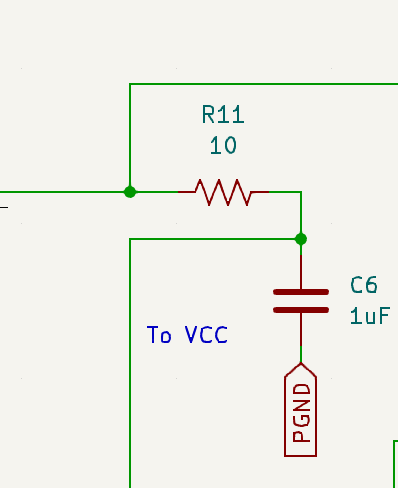
\includegraphics[scale = 0.5]{IC-filter}
	\caption{From top left to bottom right: datasheet recommendation; connection for each panel; IC damping RC circuit}
	\label{fig:mesh2}
\end{figure}



\subsection{PV-input switch}

So as to be able to control the input of the PV panels into the circuit, a manual switch is used and is followed by a voltage divider, whose output can be read on a pin out from the PCB in order to take measurements of the voltage at switch the solar panels are being made to operate at. The voltage divider output will be a third of the PV-panel operating voltage.

\subsection{Establishing the MPP}

The BQ24650 varies the current supplied to the batteries and circuit so that the operating voltage of the solar panels is mantained constant. This form of maximum power point tracking thus keeps us near the maximum power point as the IV curve of the PV panels vary according to the available illumination. 

In order to satisfy this requirement, the BQ24650 pin ``MPPSET'' provides a regulated voltage of 1.2 V.Therefore, by means of a voltage divider, it is possible to set the voltage at which the PV panels operate according to the equation:

\begin{equation}
	V_{MPPSET} = 1.2 V x (1 + \frac{R6}{R7})
\end{equation}

By choosing R6 = 120 k$\Omega$ and R7 = 30 k$\Omega$, we should set an MPP of 6V. We should try to verify if this is the optimum voltage for the solar panels once they arrive.

 The forward voltage of the PDS-1040L diodes on the PV-panel input is ~0.5 V. 
 
\subsubsection{Output of BQ24650}

As the BQ24650 is a switch-mode battery charge controller whose switching is done by external MOSFETs, we have had to implement these transistors as well as the LC filter at the output and a capacitor at its input. The full datasheet reference schematic is shown in figure \ref{fig:mesh3}.

\begin{figure}[h]
	\centering
   	 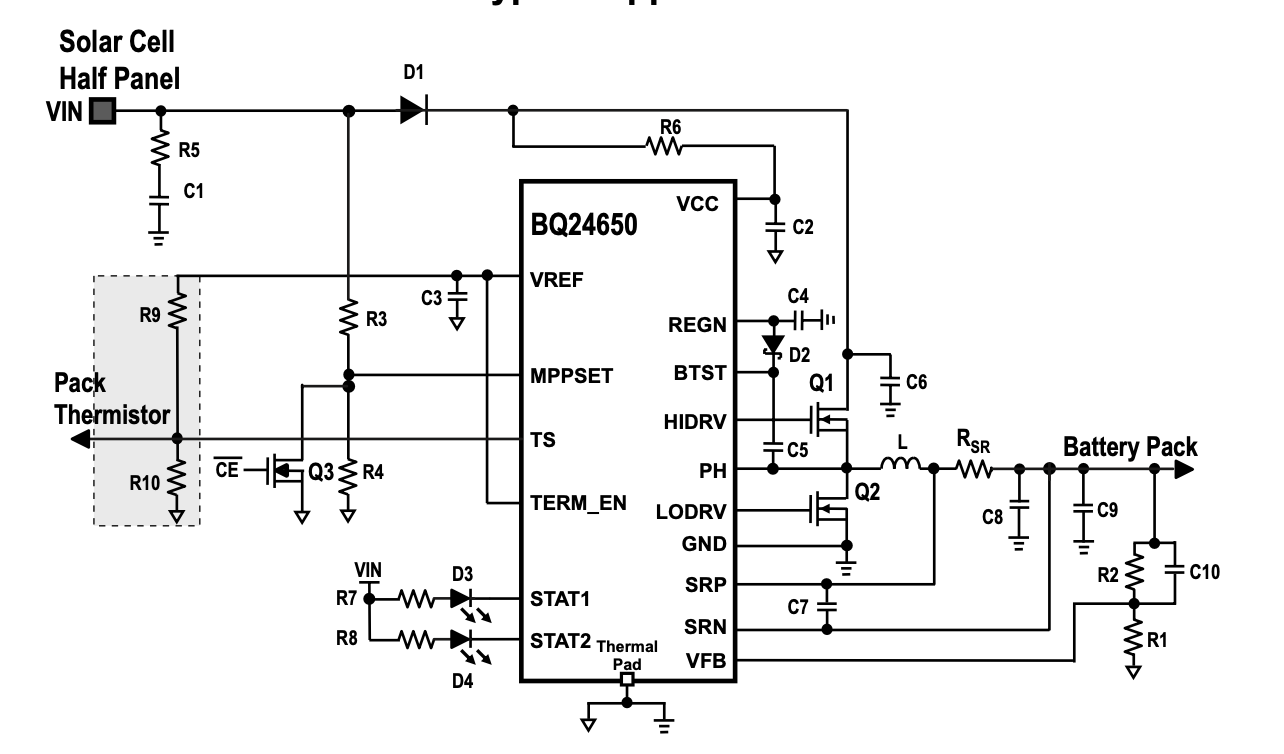
\includegraphics[width=\linewidth]{BQ24650-ref-schematic}
	\caption{BQ24650 typical application}
	\label{fig:mesh3}
\end{figure}

While this typical application has been followed and the components recommended in the datasheet have been used when implmenting the BQ26450, a few design choices were required along the way. Firstly, a 10 uF X7R input capacitor, C13 on the PCB, has been chosen. It follows the voltage-rating recommendation and but its ripple current rating is a little more opaque. According to the equation presented in the datasheet, this rating, with a duty cycle of 0.7, is 900 mA. Using the graph presented in the spec sheet of the capacitor\footnote{\href{https://ds.yuden.co.jp/TYCOMPAS/ap/detail?pn=MSASG31LAB7106KTNB25}{https://ds.yuden.co.jp/TYCOMPAS/ap/detail?pn=MSASG31LAB7106KTNB25}}., this results in a change in temperature of around 20ºC, which is within the operating temperature limit.

The output current-sensing resistor, inductor and capacitor have been chosen in accordance with table 1 of the datasheet and assuming a current of 1 A. There is, however, a strong possibility that the current may be higher than this so these components need to be reassessed once we have an energy source. The LC resonant frequency is 13 kHz, within the 12 -17 kHz band recommended by the manufacturer and the saturation current of the inductor is 13.5 A, above the 1.14 A calculated from equation 13. Finally, the output capacitors shouldn't allow excessive voltage ripple, which was calculated from equation 16 to be 31 uV. One doubt which is difficult to resolve is whether the capacitors can cope with any current ripple. However, given that the voltage ripple is low, it may be fair to assume that the capacitors can absorb the current ripple, despite not having a current ripple rating in the manufacturer's documentation. Additionally, as we have implemented other stages of voltage regulation, any ripple at this point should not affect the ICs that are ultimately supplied. 

So as to control the the voltage, and therefore the charge, of the batteries, the feedback resistors on the feedback pin of the BQ24650 are set so that the Li-ion batteries charge to 4.2 V, as per equation 1. It may be avisable to lower this to 4.1 V to extend battery lifetimes and choose resistors with a lower tolerance and possibly even a higher resistance to reduce losses.

We have chosen not to use the BQ24650's thermistor initially, although one is provided by the battery management IC and is located on the other side of the PCB. In order to ensure the operation of the BQ24650, the thermistor pin has been set at 1.96 V via a voltage divider on the $V_{REF}$ pin, which gives 59\% of  $V_{REF}$, within the limits of $V_{LTF}$ and $V_{HTF}$. It may be interesting to consider the use of the thermistor in the next version of the circuit. A switch is also placed on this pin in the typical application shown in figure \ref{fig:mesh3} and may be an option in the next version.

All other components for the BQ24650 have been chosen as from the list in table 3 of the datasheet, although the manufacturer is often not the same.

Finally, the datasheet recommends separate grounding for analogue and power, but we've implemented just a single ground, the reasons for which will be explored more fully when discussing layout.

\subsection{Battery management with the BQ76920}

Since we have decided to use economical Li-ion batteries in the buoy, it is important to understand how we can maintain the battery charge balanced so that we can optimise their lifetimes. The first step in this direction is to include the BQ76920 in this prototype to learn how to program the IC to perform this function, as well as return to the MCU information related to the power characteristics of the electronics and the battery. Even so, manual switches have been placed around this IC to permit operation without battery management. 

All the components were taken directly from the datasheet, except for the current-sense resistor. Its value was estimated by considering an overcharge discharge of approximately 4 A.

It's also convenient to note here that this IC allows for the management of up to five Li-ion batteries. Once we have more information about energy supply capabilities and demand requirements of the system, it may be advantageous to substitute the BQ76920 with the BQ76930 so that up to thirty batteries may be managed.

The BQ76920 is followed by another voltage divider to provide an analogue measurement of the battery voltage. 


\subsection{INA138 analogue current measurement}

The 100-m$\Omega$ shunt resistor will give a voltage of 200 mV for a current of 2 A, the upper limit being considered for our circuit's current requirement, well within the 500-mV limit for accurate reading of currents. Nevertheless, it may be beneficial to lower this shunt resistor's value to reduce power loss, though a concern may be accuracy when the resistor's voltage is sub-50 mV. The output resistor has been selected from the table in figure 9 of the datasheet such that a voltage gain of 5 will produce a maximum output voltage of 1 V for 24.9 k$\Omega$ resistor, assuming a 2-A current. A capacitor is placed in parallel to the output resistor in order to provide any instantaneous demand for current required at the MCU ADC, in accordance with page 12 of the datasheet. The low-pass filter formed by the resistor and capacitor gives a 3-dB bandwidth of 780 Hz. Based purely on the range in figure 13 of the datasheet, this may be too low for our purposes. Nonetheless, the aim is to only use the BQ769X0 for current-demand measurements in future versions.

\subsection{TPS564257 voltage regulator}

The TPS564257 was chosen due to the simplicity of its implmentation, low BOM and, most importantly, for being able to operate in the required intervals. The overall voltage-regulation approach is to use a voltage regulator to bring the voltage down from the battery voltage to 3.4 V, which is then lowered to 3.3 V by the LDO. The purpose is to use the efficient voltage regulator to do the majority of the lowering work and then use the LDO to achieve an accurate voltage level for the majority of the ICs. An additional, separate LDO may be required solely for the GPS module to provide it with the stablest voltage possible. Its implementation was lifted directly from the Texas Instrument's website, as shown in figure \ref{fig:mesh4}.

\begin{figure}[h]
	\centering
   	 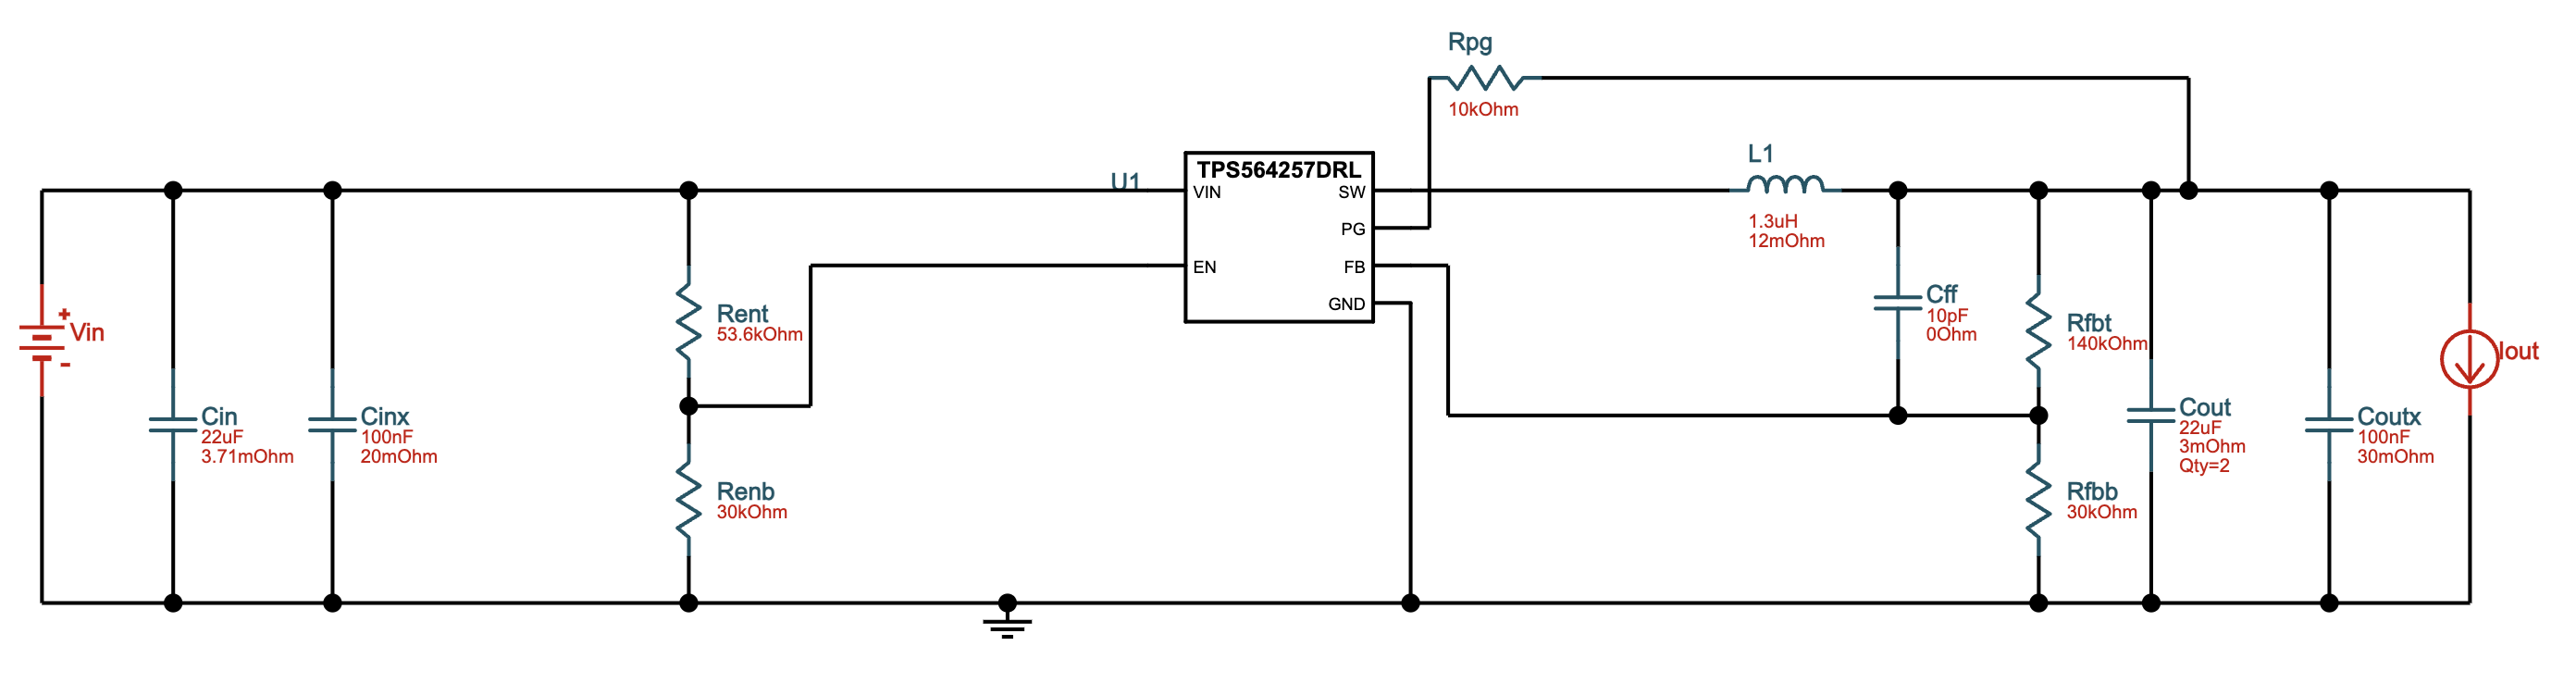
\includegraphics[width=\linewidth]{TPS564257-schematic}
	\caption{TPS564257 schematic}
	\label{fig:mesh4}
\end{figure}

\subsection{AP2112K low-dropout regulator}

Finally, the LDO implementation is taken directly from its datasheet. It is capable of only supplying up to 600 mA of output current, but higher-power functions like communications modules can be power directly from the output of the voltage regulator.

\end{document}